\documentclass[11pt,class=report,crop=false]{standalone}
\usepackage[screen]{../python}

\begin{document}


%====================================================================
\chapitre{Tenseurs}
%====================================================================

\insertvideo{XoB6xPMZ8y8}{partie 15. Tenseurs}


\objectifs{Un tenseur est un tableau à plusieurs dimensions, qui généralise la notion de matrice et de vecteur et permet de faire les calculs dans les réseaux de neurones.}


%%%%%%%%%%%%%%%%%%%%%%%%%%%%%%%%%%%%%%%%%%%%%%%%%%%%%%%%%%%%%%%%%%%%%
\section{Tenseurs (avec \numpy)}

\index{tenseur}

%--------------------------------------------------------------------
\subsection{Qu'est ce qu'un tenseur ?}

Un tenseur est un tableau de nombres à plusieurs dimensions.
Voici des exemples de tenseurs :
\begin{itemize}
  \item un vecteur $V$ est un tenseur de dimension $1$ (c'est un tableau à une seule dimension),
  \item une matrice $M$ est un tenseur de dimension $2$ (c'est un tableau à deux dimensions),
  \item un $3$-tenseur $T$ est un tableau à $3$ dimensions.
\end{itemize}

Voici un exemple pour chacune des situations avec leur définition \numpy.

\begin{minipage}{0.4\textwidth}
$$V = \begin{pmatrix}5\\7\\8\end{pmatrix}$$
\end{minipage}
\begin{minipage}{0.4\textwidth}
\begin{lstlisting}
V = np.array([5, 7, 8]) 
\end{lstlisting}
\end{minipage}

\medskip

\begin{minipage}{0.4\textwidth}
$$M = \begin{pmatrix}
6 & 0 & 2 \\ 
3 & 2 & 4 \\
\end{pmatrix}$$
\end{minipage}
\begin{minipage}{0.4\textwidth}
\begin{lstlisting}
M = np.array([[6, 0, 2], 
	          [3, 2, 4]])
\end{lstlisting}
\end{minipage}

\medskip

\begin{minipage}{0.4\textwidth}
\myfigure{0.6}{
  \tikzinput{fig-tenseur}
}
\end{minipage}
\begin{minipage}{0.4\textwidth}
\begin{lstlisting}
T = np.array([ [[5, 1, 0], 
	            [3, 3, 2]],
	           [[1, 1, 0], 
	            [5, 1, 7]], 
	           [[0, 0, 1], 
	            [8, 1, 9]] ])
\end{lstlisting}
\end{minipage}


\medskip

On accède aux éléments en utilisant les coordonnées :
\begin{itemize}
  \item $V[i]$,
  \item $M[i,j]$ (ou bien $M[i][j]$),
  \item $T[i,j,k]$ (ou bien $T[i][j][k]$).
\end{itemize}

Plus généralement un \defi{$n$-tenseur} $T$ est un tableau de nombres ayant $n$ dimensions.
On accède à ses éléments en précisant ses $n$ coordonnées $T[i_1,i_2,\ldots,i_n]$.

Il n'est pas très difficile de définir des $n$-tenseurs, ce sont juste des tableaux de nombres. Par contre, il est plus difficile de visualiser un tenseur à partir de la dimension $4$.
Une matrice peut être vue comme une liste de vecteurs. De même, un $3$-tenseur est une liste de matrices, un $4$-tenseur une liste de $3$-tenseurs\ldots

Une autre façon de voir un $4$-tenseur est de le présenter comme une matrice dans laquelle chaque élément est en fait une matrice :
$$T = \begin{pmatrix}
M_{1,1} & M_{1,2} & \cdots \\
M_{2,1} & M_{2,2} & \cdots \\
\vdots & \vdots   & \vdots \\
\end{pmatrix}.$$



\begin{remarque*}
\sauteligne
\begin{itemize}

  \item La notion de tenseur avec \tensorflow{} est beaucoup plus sophistiquée que celle de tenseur avec \numpy. Nous en aurons un aperçu dans la section suivante.
  
  \item Il existe une définition plus générale (et beaucoup plus compliquée) de tenseur en mathématiques. Pour ceux qui connaissent les espaces vectoriels, la différence entre un tenseur mathématique et un tenseur comme présenté ici est la même qu'entre une application linéaire et une matrice.
\end{itemize}

\end{remarque*}


%--------------------------------------------------------------------
\subsection{Vocabulaire}


Il est important de maîtriser le vocabulaire lié aux tenseurs et de ne pas confondre les notions.

\begin{itemize}
  \item \defi{Dimension}. 
  \begin{itemize}
    \item C'est le nombre d'indices qu'il faut utiliser pour accéder à un élément. 
    Chaque indice correspond à un \defi{axe}.
    \item Un vecteur est de dimension $1$, une matrice de dimension $2$ (le premier axe correspond par exemple aux lignes et le second axe aux colonnes), un $n$-tenseur est de dimension $n$ car on accède à un élément $T[i_1,i_2,\ldots,i_n]$ en utilisant $n$ indices.
    \item Le nom anglais est \emph{rank} (qui n'a rien à voir avec le rang d'une matrice).   
    \item La commande est \ci{T.ndim}.
 \end{itemize}
  
  \item \defi{Taille}.
    \begin{itemize}
      \item C'est la liste des longueurs de chaque axe.
      \item Un vecteur de longueur $3$ a pour taille $(3)$ que l'on note plutôt $(3,)$ (pour signifier que c'est bien une liste). Une matrice $3\times 4$ a pour taille $(3,4)$. Un tenseur de taille $(3,5,7,11)$ est un tenseur de dimension $4$, le premier indice $i_1$ varie de $1$ à $3$ (ou plutôt de $0$ à $2$ avec \Python), le second indice $i_2$ varie de $1$ à $5$\ldots
      \item Le nom anglais est \emph{shape}.     
      \item La commande est \ci{T.shape}.\index{numpy@\numpy!shape@\ci{shape()}}
    \end{itemize}
    
  
  \item \defi{Nombre d'éléments}.
    \begin{itemize}
      \item C'est le nombre total d'éléments nécessaire pour définir un tenseur. Cela correspond au nombre d'emplacements qu'il faut réserver dans la mémoire pour stocker le tenseur. Le nombre d'éléments d'un tenseur est le produit $\ell_1 \times \cdots \times \ell_n$ des longueurs de la taille $(\ell_1,\ldots,\ell_n)$ du tenseur.
      \item Un vecteur de longueur $3$ possède $3$ éléments, une matrice $3\times 4$ en a $12$ et un $4$-tenseur de taille $(3,5,7,11)$ en a $3\times5\times7\times 11$.
      \item Le nom anglais est \emph{size}.       
      \item La commande est \ci{T.size}.

    \end{itemize}    
\end{itemize}      
    

Voici des exemples que l'on a déjà rencontrés :
\begin{itemize}
  \item Une image $28\times28$ en niveaux de gris est représentée par un tenseur de taille $(28, 28)$. 
  Sa dimension est $2$ et son nombre d'éléments est $784 = 28 \times 28$.
\item Une image $32\times32$ en couleurs est représentée par un tenseur de taille $(32, 32,3)$. Sa dimension est $3$ et son nombre d'éléments est $3072 = 32 \times 32 \times 3$.
\item Les données d'apprentissage de la base CIFAR-10 sont composées de $50\,000$ images couleurs de taille $32\times32$. L'ensemble des données est donc représenté par un $4$-tenseur de taille $(50\,000,32,32,3)$. Un pixel étant codé par un entier sur un octet, il faut réserver $50\,000 \times 32 \times 32 \times 3 = 153.6$ Mo en mémoire.
\end{itemize}


%--------------------------------------------------------------------
\subsection{Opérations sur les tenseurs}

Les tenseurs se comportent comme les vecteurs et les tableaux \numpy{} vus dans les chapitres \og{}Python : numpy et matplotlib avec une variable\fg{}
et \og{}Python : numpy et matplotlib avec deux variables\fg{}.

Nous reprenons les exemples définis plus haut.

\textbf{Opérations sur tous les éléments.}
\begin{itemize}
  \item \ci{V + 3} ajoute $3$ à chaque élément de \ci{V}.
  \item \ci{A ** 2} calcule le carré de chaque élément de \ci{A}.
  \item \ci{T - 1} retranche $1$ à chaque élément de \ci{T}.
\end{itemize}

\textbf{Opérations élément par élément entre tenseurs de même taille.}
\begin{itemize}
  \item \ci{A * AA} calcule chaque produit $a_{ij}\times a'_{ij}$ (ici en dimension 2) et n'a rien à voir avec le produit de deux matrices.
  \item \ci{T + TT} calcule chaque somme $T_{ijk}+T'_{ijk}$ (ici en dimension 3).
\end{itemize}

\textbf{Fonctions sur un tenseur.}

Certaines fonctions agissent élément par élément d'autre pas.
\begin{itemize}
  \item \ci{V.mean()} renvoie la moyenne de tous les éléments.
  \item \ci{A.sum()} renvoie la somme de tous les éléments.
  \item \ci{np.sqrt(T)} renvoie un tenseur, où chaque élément est obtenu par racine carrée.
\end{itemize}


%--------------------------------------------------------------------
\subsection{Changer de taille}

Changer la taille d'un tenseur tout en conservant le nombre d'éléments est un opération fréquente.

\textbf{Aplatissement.} 
C'est la mise sous la forme d'un vecteur (tenseur de dimension $1$). 
L'instruction est \ci{T.flatten()}\index{numpy@\numpy!flatten@\ci{flatten()}} qui pour notre exemple du début de chapitre renvoie le tenseur de taille $(18,)$ :
\mycenterline{\ci{[5 1 0 3 3 2 1 1 0 5 1 7 0 0 1 8 1 9]}}

\textbf{Changement de taille.}
La méthode \ci{reshape()}\index{tf@\tensorflow/\keras!reshape@\ci{reshape()}} transforme un tenseur en changeant sa taille.
Par exemple notre tenseur \ci{T} est de taille $(3,2,3)$ et possède $18$ éléments.
\begin{itemize}
  \item \ci{T1 = np.reshape(T,(2,9))} renvoie un tenseur de taille $(2,9)$ contenant les éléments de \ci{T} réorganisés.

\begin{center}
\begin{minipage}{0.5\textwidth}  
\begin{lstlisting}
[[5 1 0 3 3 2 1 1 0]
 [5 1 7 0 0 1 8 1 9]]  
\end{lstlisting}
\end{minipage}
\end{center}
  
  \item \ci{T2 = np.reshape(T,(2,3,3))} renvoie un tenseur de taille $(2,3,3)$.
\begin{center}
\begin{minipage}{0.5\textwidth}    
\begin{lstlisting}
[[[5 1 0]
  [3 3 2]
  [1 1 0]]
 [[5 1 7]
  [0 0 1]
  [8 1 9]]]      
\end{lstlisting}
\end{minipage}
\end{center}  
  \item \ci{T3 = np.reshape(T,(9,-1))} renvoie un tenseur de taille $(9,2)$. Le \og{}\ci{-1}\fg{} indique à \Python{} qu'il doit deviner tout seul la taille à calculer (sachant qu'il y a $18$ éléments une taille $(9,x)$ impose $x=2$).
\begin{center}
\begin{minipage}{0.5\textwidth}    
\begin{lstlisting}
[[5 1]
 [0 3]
 [3 2]
 [1 1]
 [0 5]
 [1 7]
 [0 0]
 [1 8]
 [1 9]]  
\end{lstlisting}  
\end{minipage}
\end{center}
  
\end{itemize}



\textbf{Regrouper deux tenseurs.}
Soient 
$$A = \begin{pmatrix}
1 & 2 & 3 \\
4 & 5 & 6
\end{pmatrix}
\qquad\qquad
B = \begin{pmatrix}
 7 &  8 &  9 \\
10 & 11 & 12
\end{pmatrix}
$$
définis par
\begin{lstlisting}
A = np.arange(1,7).reshape((2,3))
B = np.arange(7,13).reshape((2,3))
\end{lstlisting}
Voici deux commandes illustrant le regroupement de $A$ et $B$ : 
\begin{lstlisting}
C1 = np.concatenate((A, B), axis=0)
C2 = np.concatenate((A, B), axis=1)
\end{lstlisting}

$$C_1 = \begin{pmatrix}
 1 & 2 & 3 \\
 4 & 5 & 6 \\
 7 & 8 & 9 \\
10 & 11 & 12
\end{pmatrix}
\qquad\quad
C_2 = \begin{pmatrix}
 1 & 2 & 3 & 7 & 8 & 9 \\
 4 & 5 & 6 & 10 & 11 & 12
\end{pmatrix}
$$

\bigskip

De façon plus générale, toutes les opérations dont vous pourriez avoir besoin sont disponibles, mais il faudra parfois se creuser la tête pour comprendre les mécanismes associés dès que la dimension est plus grande que $3$.


%%%%%%%%%%%%%%%%%%%%%%%%%%%%%%%%%%%%%%%%%%%%%%%%%%%%%%%%%%%%%%%%%%%%%
\section{Tenseurs (avec \tensorflow/\keras)}

Avec \tensorflow/\keras{} les tenseurs sont des objets beaucoup plus puissants que les tableaux \numpy. Il est en effet possible de manipuler des tenseurs sans définir leurs éléments. 
Nous ne voyons ici que quelques fonctionnalités, les plus simples.

%--------------------------------------------------------------------
\subsection{Une case vide}

Avec \Python{} on ne peut pas écrire l'opération
\mycenterline{\ci{y = x + 2}}
si on n'a pas auparavant affecté une valeur à la variable \ci{x}.

Ce que l'on voudrait, c'est pouvoir manipuler \ci{y} comme une variable ordinaire. Un autre point de vue est de dire que l'on veut définir la fonction $x \mapsto y = x+2$. Ainsi, on pourrait ne préciser qu'en fin de programme que la variable, ici $x$, valait en fait $7$ et donc que tout ce qui concernait $y$ l'était finalement pour $y=9$.

Voici comment faire avec \keras.

\begin{lstlisting}
from tensorflow.keras import backend as K
x = K.placeholder(shape=(1,))
y = x + 2 
f = K.function([x],[y])
print(f([7]))
\end{lstlisting}

La fonction \ci{placeholder()} réserve un emplacement mémoire pour un tenseur nommé $x$ (ici un vecteur de longueur $1$, donc un nombre), que l'on peut manipuler ensuite comme une variable.
On définit ensuite la fonction $f : x \mapsto y = x+2$. 
Ce n'est qu'à la fin, lorsque l'on calcule $f(7)$ que l'emplacement mémoire de \ci{x} est affecté à  la valeur \ci{[7]} et que le calcul $y=x+2$ est vraiment effectué. 

\bigskip
Voici un autre autre exemple qui correspond au calcul $A \times X$ où $A$ est une matrice $3\times 3$ et $X$ un vecteur de taille $3$.

\begin{lstlisting}
import numpy as np

A = K.placeholder(shape=(3,3))
X = K.placeholder(shape=(3,1))
Y = K.dot(A,X)
f = K.function([A, X], [Y])

Aval = np.arange(1,10).reshape((3,3))
Xval = np.arange(1,4).reshape((3,1))

Yval = f([Aval, Xval])
\end{lstlisting}

%--------------------------------------------------------------------
\subsection{Gradient}

\index{gradient}

On termine par une fonction de \keras{} particulièrement importante pour ce cours : la fonction gradient.

\textbf{Une variable.}

Voici comment calculer la dérivée de la fonction $x \mapsto y=x^2$ en $x_0=3$.
\begin{lstlisting}
x = K.constant([3])
y = x**2
grad = K.gradients(y, x)
print("Dérivée :", K.eval(grad[0]))
\end{lstlisting}


Voici comment calculer la dérivée de la fonction définie par $f(x) = 2\ln(x)+\exp(-x)$ en plusieurs points.

\begin{lstlisting}
def f(x):
	return 2*K.log(x) + K.exp(-x)

X = K.arange(1,4,0.5)
Y = f(X)
grad = K.gradients(Y, X)

print("Point x :", K.eval(X))
print("Valeur y=f(x) :", K.eval(Y))
print("Dérivée f'(x) :", K.eval(grad[0]))
\end{lstlisting}

Ici les abscisses $x$ sont les éléments de la liste $[1., 1.5, 2., 2.5, 3., 3.5]$,
les valeurs calculées $y=f(x)$ sont $[0.367, 1.034, \ldots ]$.
Et on obtient la liste des dérivées $f'(x)$ : $[1.632,  1.110, \ldots]$.


Avec plus de points, on trace le graphe de $f$ et sa dérivée $f'$ sur l'intervalle $[1,4]$.
\begin{center}
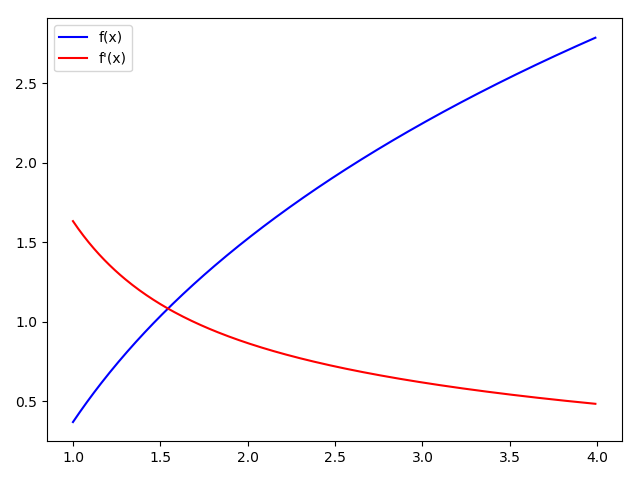
\includegraphics[scale=\myscale,scale=0.6]{figures/tenseur-derivee}
\end{center}


\textbf{Deux variables.}

Voici comment calculer le gradient de $f(x,y) = xy^2$ en $(x_0,y_0)= (2,3)$.

\begin{lstlisting}
x = K.constant([2])
y = K.constant([3])
z = x * (y**2) 
grad = K.gradients(z, [x,y])
dxZ = K.eval(grad[0])
dyZ = K.eval(grad[1])
print("Gradient :", dxZ, dyZ)
\end{lstlisting}


On peut ainsi tracer le gradient en chaque point du plan. Ci-dessous le gradient et les lignes de niveau de la fonction $f(x,y) = x^2-y^2$ (un point-selle).
\begin{center}
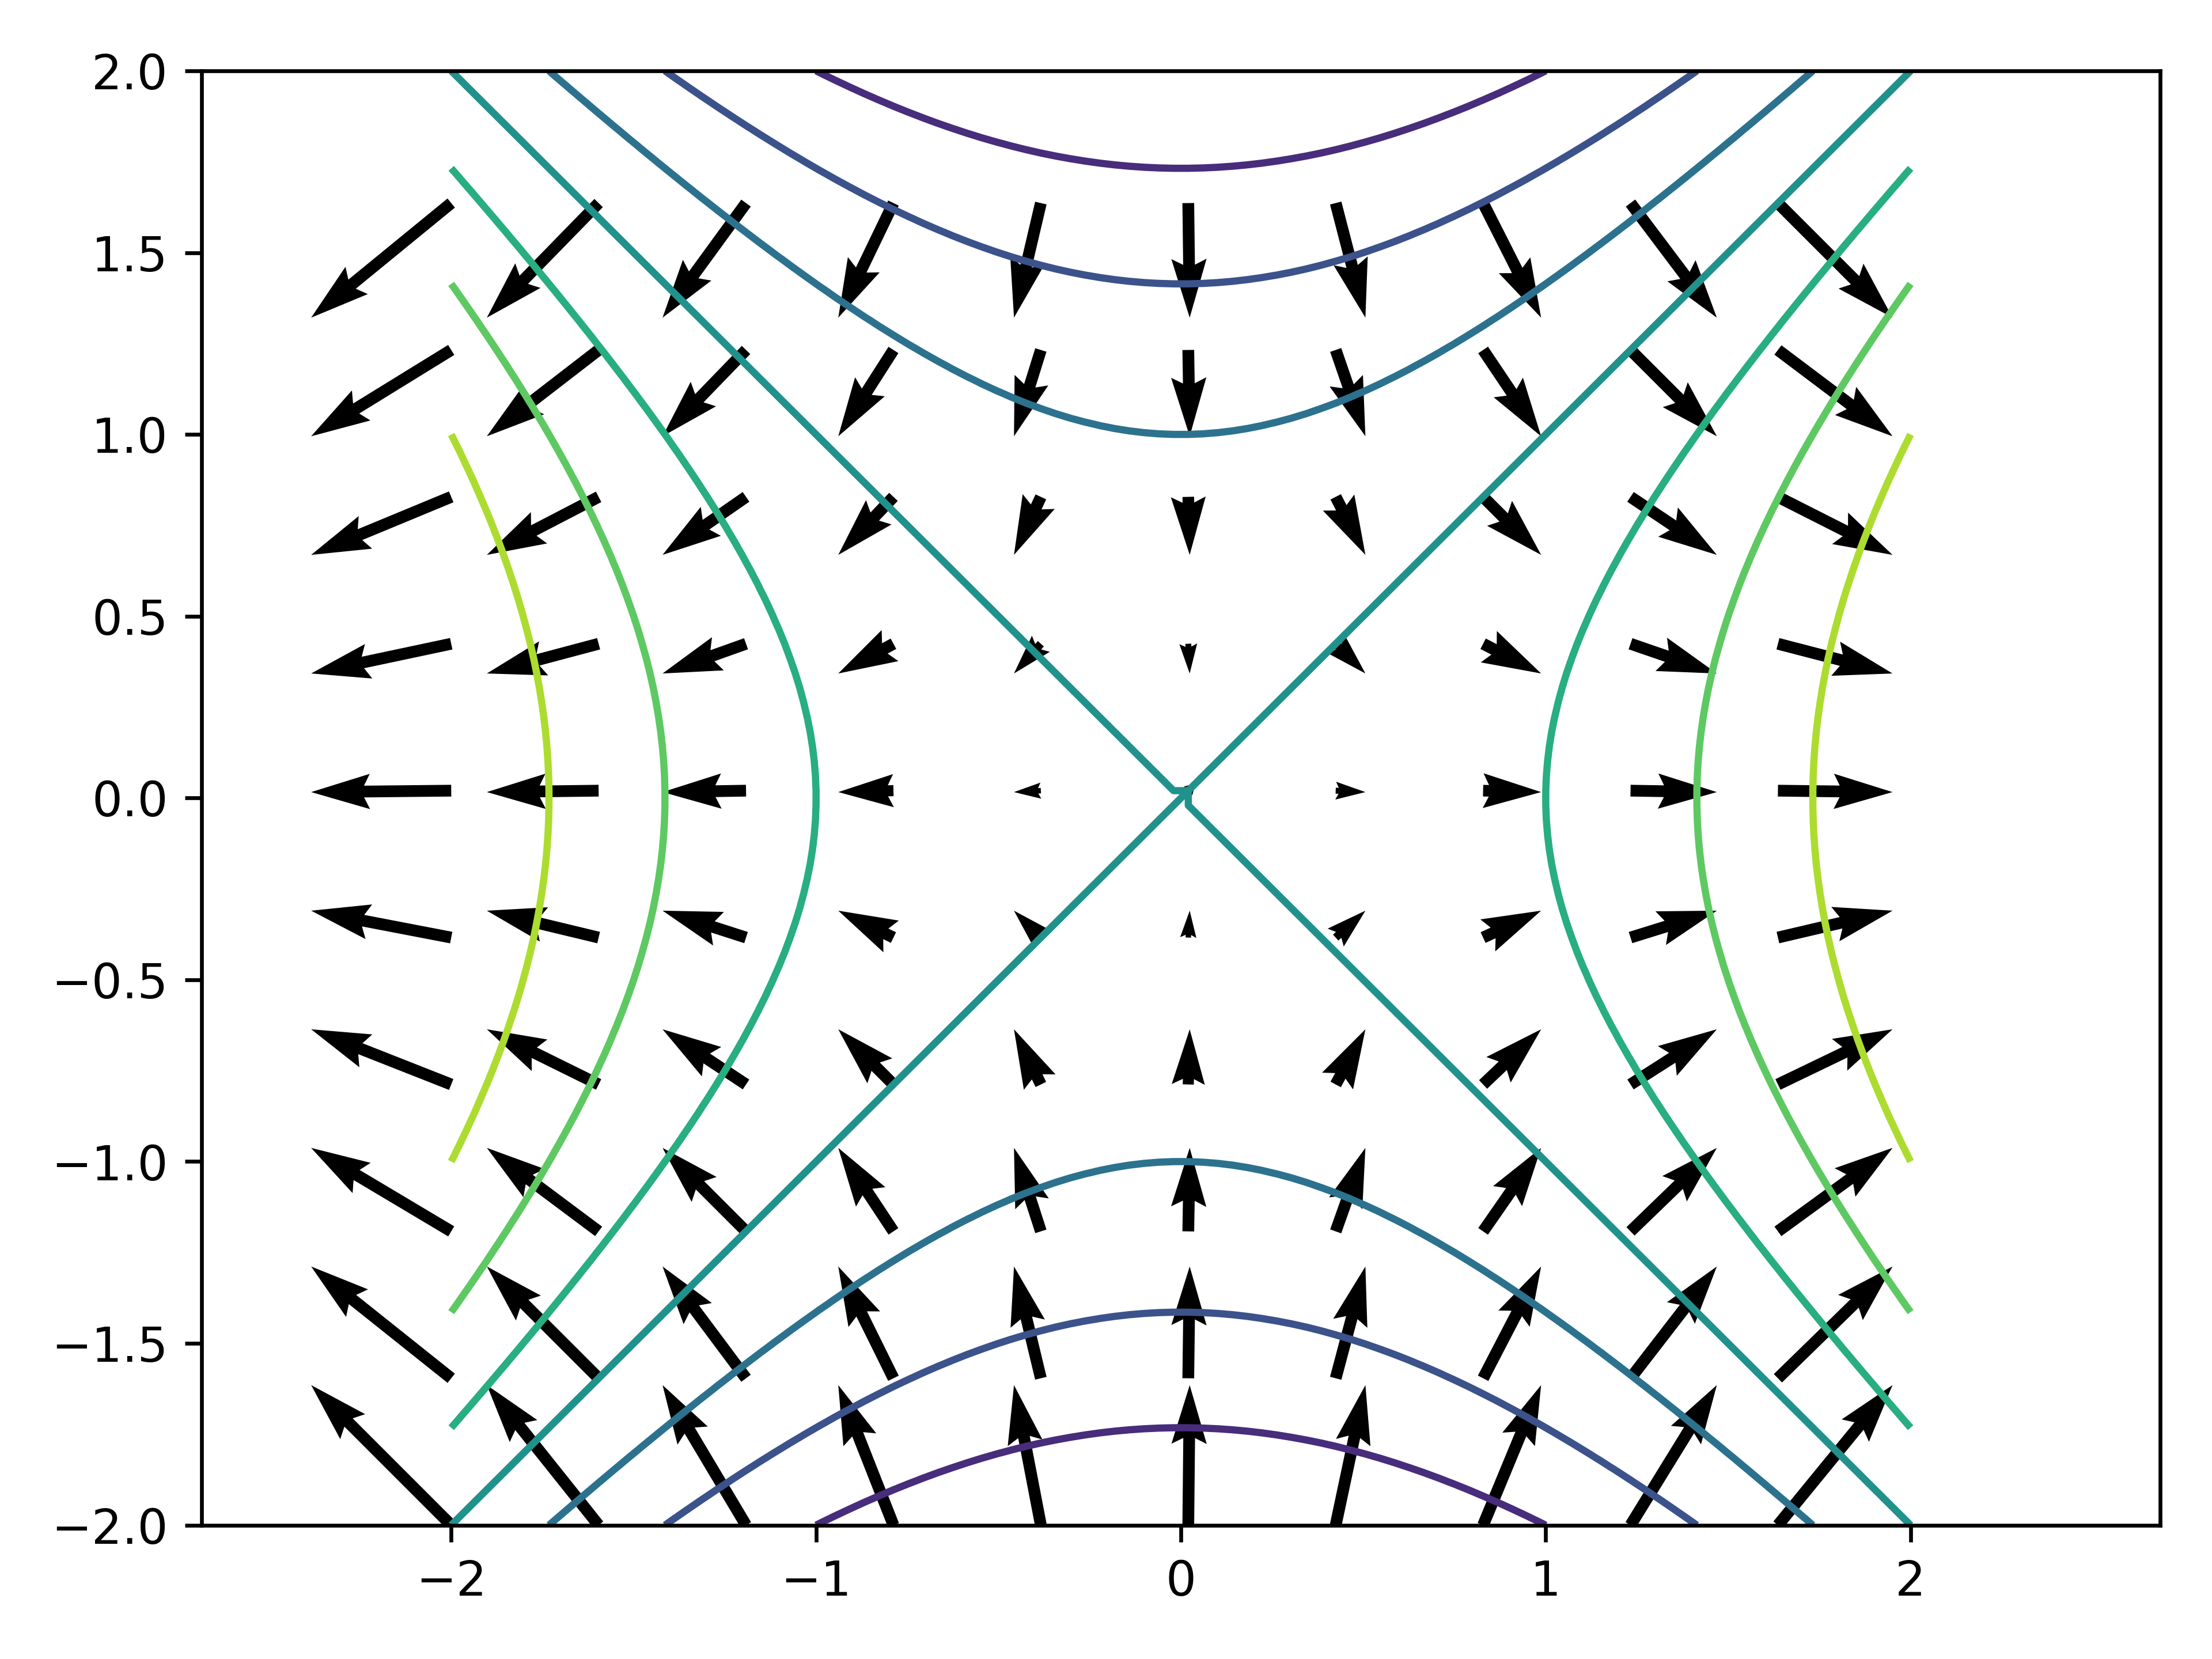
\includegraphics[scale=\myscale,scale=0.8]{figures/tenseur-gradient}
\end{center}

\end{document}
